\documentclass{article}\usepackage[]{graphicx}\usepackage[]{xcolor}
% maxwidth is the original width if it is less than linewidth
% otherwise use linewidth (to make sure the graphics do not exceed the margin)
\makeatletter
\def\maxwidth{ %
  \ifdim\Gin@nat@width>\linewidth
    \linewidth
  \else
    \Gin@nat@width
  \fi
}
\makeatother

\definecolor{fgcolor}{rgb}{0.345, 0.345, 0.345}
\newcommand{\hlnum}[1]{\textcolor[rgb]{0.686,0.059,0.569}{#1}}%
\newcommand{\hlstr}[1]{\textcolor[rgb]{0.192,0.494,0.8}{#1}}%
\newcommand{\hlcom}[1]{\textcolor[rgb]{0.678,0.584,0.686}{\textit{#1}}}%
\newcommand{\hlopt}[1]{\textcolor[rgb]{0,0,0}{#1}}%
\newcommand{\hlstd}[1]{\textcolor[rgb]{0.345,0.345,0.345}{#1}}%
\newcommand{\hlkwa}[1]{\textcolor[rgb]{0.161,0.373,0.58}{\textbf{#1}}}%
\newcommand{\hlkwb}[1]{\textcolor[rgb]{0.69,0.353,0.396}{#1}}%
\newcommand{\hlkwc}[1]{\textcolor[rgb]{0.333,0.667,0.333}{#1}}%
\newcommand{\hlkwd}[1]{\textcolor[rgb]{0.737,0.353,0.396}{\textbf{#1}}}%
\let\hlipl\hlkwb

\usepackage{framed}
\makeatletter
\newenvironment{kframe}{%
 \def\at@end@of@kframe{}%
 \ifinner\ifhmode%
  \def\at@end@of@kframe{\end{minipage}}%
  \begin{minipage}{\columnwidth}%
 \fi\fi%
 \def\FrameCommand##1{\hskip\@totalleftmargin \hskip-\fboxsep
 \colorbox{shadecolor}{##1}\hskip-\fboxsep
     % There is no \\@totalrightmargin, so:
     \hskip-\linewidth \hskip-\@totalleftmargin \hskip\columnwidth}%
 \MakeFramed {\advance\hsize-\width
   \@totalleftmargin\z@ \linewidth\hsize
   \@setminipage}}%
 {\par\unskip\endMakeFramed%
 \at@end@of@kframe}
\makeatother

\definecolor{shadecolor}{rgb}{.97, .97, .97}
\definecolor{messagecolor}{rgb}{0, 0, 0}
\definecolor{warningcolor}{rgb}{1, 0, 1}
\definecolor{errorcolor}{rgb}{1, 0, 0}
\newenvironment{knitrout}{}{} % an empty environment to be redefined in TeX

\usepackage{alltt}
\usepackage[a4paper, total={6.5in, 10.5in}]{geometry}

\author{Katarzyna Macioszek, Ada Majchrzak}
\title{Data Mining project - part I}
\IfFileExists{upquote.sty}{\usepackage{upquote}}{}
\begin{document}
\maketitle

\section{Introduction}

In this project, we will use data mining methods to perform analysis of \textit{Spambase}
dataset. The considered dataset was created from two collections of e-mails, 
the first being a set of non-spam personal and professional e-mails, and the 
second one coming from individuals who had filed spam. The e-mails were 
analyzed in terms of frequency of appearance of 54 selected words, numbers and characters,
and also in terms of the number of capital letters present. 
Those statistics were then collected into table and each record was labeled 
as spam or non-spam. Our goal is to first extract interesting and insightful data characteristics
by Exploratory Data Analysis procedures (plots, summary statistics), and then to perform a classification task,
distinguishing spam from non-spam. For the second part, we will compare the performance
of several methods, namely Linear Discriminant Analysis (LDA), Quadratic Discriminant Analysis (QDA),
K-Nearest Neighbours (KNN), and Random Forest. We will also evaluate those methods on different sets of features.
The benefit from this kind of study could be obtaining a model effective in terms 
of spam filtering. We know that spam e-mails are a very common problem in modern 
world, and although every mailbox nowadays has built-in filter for that kind
of content, non of them are completely accurate, so it is certainly a good idea
to keep studying this topic.

\section{Exploratory Data Analysis}



\subsection*{Dataset description}

The dataset consist of 4601 records, none of which contain any missing values.
There are 57 numerical features and one categorical, \textit{type}, being a target class.
The target class takes two values -- spam and nonspam. As we can see from Figure \ref{fig1},
the classes are quite well balanced. Around 60\% of the records fall into nonspam category,
and about 40\% of them are spam. As for the numerical features, they can be divided into two
groups -- 54 features containing information about the frequency of selected words, numbers and 
special characters, expressed as percentage (further called Frequency features), 
and 3 features containing information about the capital letters in the e-mail (further called Capital features):

\begin{itemize}
  \item capitalAve -- average length of an uninterrupted sequence of capital letters,
  \item capitalLong -- length of longest uninterrupted sequence of capital letters,
  \item capitalTotal -- total number of capital letters.
\end{itemize}
Basic summary statistics for the numerical features can be found in Table \ref{tab1}.
The maximum frequency found in the dataset equals 42.8, and it is observed for \textit{num3d} variable. 
In general, the values for Frequency features are really low -- in most of the cases, even the $3^{rd}$
quartile is very close to 0, or even equal to 0, which suggest that the identification of 
potential outliers might prove challenging. There are only two variables of that type
for which the $3^{rd}$ quartile exceeds 1 -- \textit{you} (2.6) and \textit{your} (1.3).
Of course, this data stucture results in quite small standard deviations for the Frequency features.
Regarding Capital features, here the range of values is significantly broader. The minimum for all
three of those is 1, while the maximum is 1102.5 for \textit{capitalAve}, 9989.0 for \textit{capitalLong},
and 15841.0 for \textit{capitalTotal}. As expected, also the standard deviations for this set
of features are much higher compared to the previous one. Those differences need to be
kept in mind and accounted for during the classfication tasks by appropriate data transformations.



\begin{knitrout}
\definecolor{shadecolor}{rgb}{0.969, 0.969, 0.969}\color{fgcolor}\begin{figure}[h]
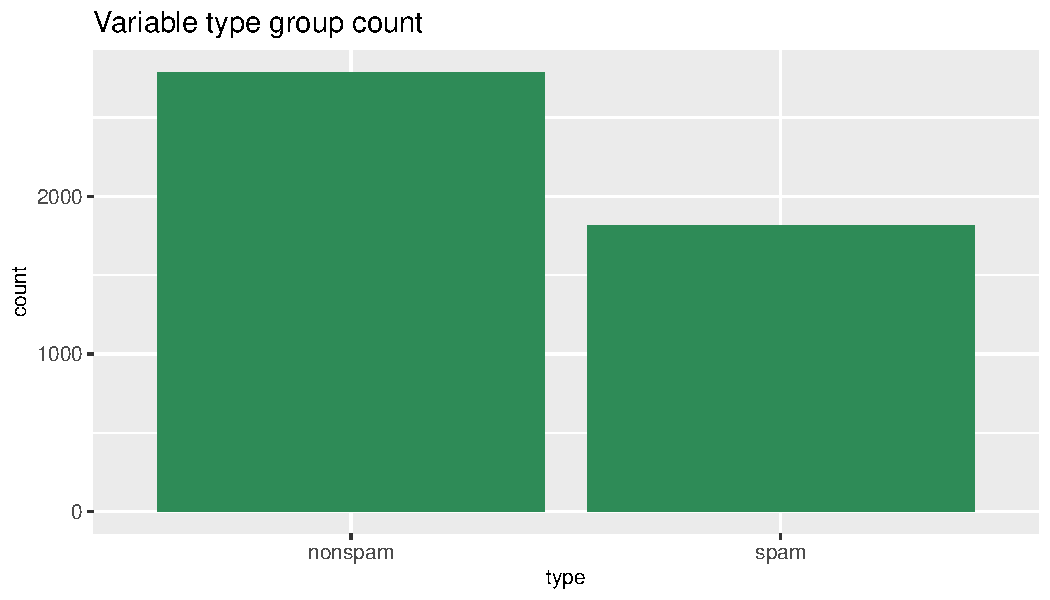
\includegraphics[width=\maxwidth]{figure/tgtClassPlot-1} \caption[\label{fig1} Target class distribution]{\label{fig1} Target class distribution}\label{fig:tgtClassPlot}
\end{figure}

\end{knitrout}


% latex table generated in R 4.3.1 by xtable 1.8-4 package
% Wed Dec  6 19:58:32 2023
\begin{table}[ht]
\centering
\begin{tabular}{rrrrrrrr}
  \hline
 & Mean & Std.Dev & Min & Max & Q1 & Median & Q3 \\ 
  \hline
address & 0.21 & 1.29 & 0.00 & 14.28 & 0.00 & 0.00 & 0.00 \\ 
  addresses & 0.05 & 0.26 & 0.00 & 4.41 & 0.00 & 0.00 & 0.00 \\ 
  all & 0.28 & 0.50 & 0.00 & 5.10 & 0.00 & 0.00 & 0.42 \\ 
  business & 0.14 & 0.44 & 0.00 & 7.14 & 0.00 & 0.00 & 0.00 \\ 
  capitalAve & 5.19 & 31.73 & 1.00 & 1102.50 & 1.59 & 2.28 & 3.71 \\ 
  capitalLong & 52.17 & 194.89 & 1.00 & 9989.00 & 6.00 & 15.00 & 43.00 \\ 
  capitalTotal & 283.29 & 606.35 & 1.00 & 15841.00 & 35.00 & 95.00 & 266.00 \\ 
  charDollar & 0.08 & 0.25 & 0.00 & 6.00 & 0.00 & 0.00 & 0.05 \\ 
  charExclamation & 0.27 & 0.82 & 0.00 & 32.48 & 0.00 & 0.00 & 0.32 \\ 
  charHash & 0.04 & 0.43 & 0.00 & 19.83 & 0.00 & 0.00 & 0.00 \\ 
  charRoundbracket & 0.14 & 0.27 & 0.00 & 9.75 & 0.00 & 0.06 & 0.19 \\ 
  charSemicolon & 0.04 & 0.24 & 0.00 & 4.38 & 0.00 & 0.00 & 0.00 \\ 
  charSquarebracket & 0.02 & 0.11 & 0.00 & 4.08 & 0.00 & 0.00 & 0.00 \\ 
  conference & 0.03 & 0.29 & 0.00 & 10.00 & 0.00 & 0.00 & 0.00 \\ 
  credit & 0.09 & 0.51 & 0.00 & 18.18 & 0.00 & 0.00 & 0.00 \\ 
  cs & 0.04 & 0.36 & 0.00 & 7.14 & 0.00 & 0.00 & 0.00 \\ 
  data & 0.10 & 0.56 & 0.00 & 18.18 & 0.00 & 0.00 & 0.00 \\ 
  direct & 0.06 & 0.35 & 0.00 & 4.76 & 0.00 & 0.00 & 0.00 \\ 
  edu & 0.18 & 0.91 & 0.00 & 22.05 & 0.00 & 0.00 & 0.00 \\ 
  email & 0.18 & 0.53 & 0.00 & 9.09 & 0.00 & 0.00 & 0.00 \\ 
  font & 0.12 & 1.03 & 0.00 & 17.10 & 0.00 & 0.00 & 0.00 \\ 
  free & 0.25 & 0.83 & 0.00 & 20.00 & 0.00 & 0.00 & 0.10 \\ 
  george & 0.77 & 3.37 & 0.00 & 33.33 & 0.00 & 0.00 & 0.00 \\ 
  hp & 0.55 & 1.67 & 0.00 & 20.83 & 0.00 & 0.00 & 0.00 \\ 
  hpl & 0.27 & 0.89 & 0.00 & 16.66 & 0.00 & 0.00 & 0.00 \\ 
  internet & 0.11 & 0.40 & 0.00 & 11.11 & 0.00 & 0.00 & 0.00 \\ 
  lab & 0.10 & 0.59 & 0.00 & 14.28 & 0.00 & 0.00 & 0.00 \\ 
  labs & 0.10 & 0.46 & 0.00 & 5.88 & 0.00 & 0.00 & 0.00 \\ 
  mail & 0.24 & 0.64 & 0.00 & 18.18 & 0.00 & 0.00 & 0.16 \\ 
  make & 0.10 & 0.31 & 0.00 & 4.54 & 0.00 & 0.00 & 0.00 \\ 
  meeting & 0.13 & 0.77 & 0.00 & 14.28 & 0.00 & 0.00 & 0.00 \\ 
  money & 0.09 & 0.44 & 0.00 & 12.50 & 0.00 & 0.00 & 0.00 \\ 
  num000 & 0.10 & 0.35 & 0.00 & 5.45 & 0.00 & 0.00 & 0.00 \\ 
  num1999 & 0.14 & 0.42 & 0.00 & 6.89 & 0.00 & 0.00 & 0.00 \\ 
  num3d & 0.07 & 1.40 & 0.00 & 42.81 & 0.00 & 0.00 & 0.00 \\ 
  num415 & 0.05 & 0.33 & 0.00 & 4.76 & 0.00 & 0.00 & 0.00 \\ 
  num650 & 0.12 & 0.54 & 0.00 & 9.09 & 0.00 & 0.00 & 0.00 \\ 
  num85 & 0.11 & 0.53 & 0.00 & 20.00 & 0.00 & 0.00 & 0.00 \\ 
  num857 & 0.05 & 0.33 & 0.00 & 4.76 & 0.00 & 0.00 & 0.00 \\ 
  order & 0.09 & 0.28 & 0.00 & 5.26 & 0.00 & 0.00 & 0.00 \\ 
  original & 0.05 & 0.22 & 0.00 & 3.57 & 0.00 & 0.00 & 0.00 \\ 
  our & 0.31 & 0.67 & 0.00 & 10.00 & 0.00 & 0.00 & 0.38 \\ 
  over & 0.10 & 0.27 & 0.00 & 5.88 & 0.00 & 0.00 & 0.00 \\ 
  parts & 0.01 & 0.22 & 0.00 & 8.33 & 0.00 & 0.00 & 0.00 \\ 
  people & 0.09 & 0.30 & 0.00 & 5.55 & 0.00 & 0.00 & 0.00 \\ 
  pm & 0.08 & 0.43 & 0.00 & 11.11 & 0.00 & 0.00 & 0.00 \\ 
  project & 0.08 & 0.62 & 0.00 & 20.00 & 0.00 & 0.00 & 0.00 \\ 
  re & 0.30 & 1.01 & 0.00 & 21.42 & 0.00 & 0.00 & 0.11 \\ 
  receive & 0.06 & 0.20 & 0.00 & 2.61 & 0.00 & 0.00 & 0.00 \\ 
  remove & 0.11 & 0.39 & 0.00 & 7.27 & 0.00 & 0.00 & 0.00 \\ 
  report & 0.06 & 0.34 & 0.00 & 10.00 & 0.00 & 0.00 & 0.00 \\ 
  table & 0.01 & 0.08 & 0.00 & 2.17 & 0.00 & 0.00 & 0.00 \\ 
  technology & 0.10 & 0.40 & 0.00 & 7.69 & 0.00 & 0.00 & 0.00 \\ 
  telnet & 0.06 & 0.40 & 0.00 & 12.50 & 0.00 & 0.00 & 0.00 \\ 
  will & 0.54 & 0.86 & 0.00 & 9.67 & 0.00 & 0.10 & 0.80 \\ 
  you & 1.66 & 1.78 & 0.00 & 18.75 & 0.00 & 1.31 & 2.64 \\ 
  your & 0.81 & 1.20 & 0.00 & 11.11 & 0.00 & 0.22 & 1.27 \\ 
   \hline
\end{tabular}
\caption{Summary statistics for numerical features} 
\label{tab1}
\end{table}


\subsection*{Potential outliers}

As we already mentioned, the distribution observed for the Frequency features is quite peculiar,
with all three quartiles equal to zero in most cases. For that reason, finding the
potential outliers migth be problematic -- for sure the classical approach with $1.5IQR$
would not be a good idea here, as it could missclassify most of the nonzero observations 
as outliers. Moreover, given the characteristics of our data, even the unusually high
frequencies don't necessarily need to be treated as outliers causing biased results
in data analysis or classification task. On the contrary, we expect that they can be 
quite informative when trying to distinguish between spam and nonspam e-mails, as 
some of the words or characters will not be used much in private messages, but repeated
frequently in spam, and vice versa. Considering all that, we will not try to identify and 
remove the potential outliers, but we will use boxplots to see how various transformations
will influence data distribution and the number of detected potential oultiers. Of course, 
as we have 54 Frequency features, we will not show the boxplots for all of them.
Instead, we picked three variables with the widest range of values - \textit{george},
\textit{num3d} and \textit{charExclamation}. As for the data transformations, 
we will compare z-score standardization and $\log(x+0.1)$ transformation.



\begin{knitrout}
\definecolor{shadecolor}{rgb}{0.969, 0.969, 0.969}\color{fgcolor}\begin{figure}[h]
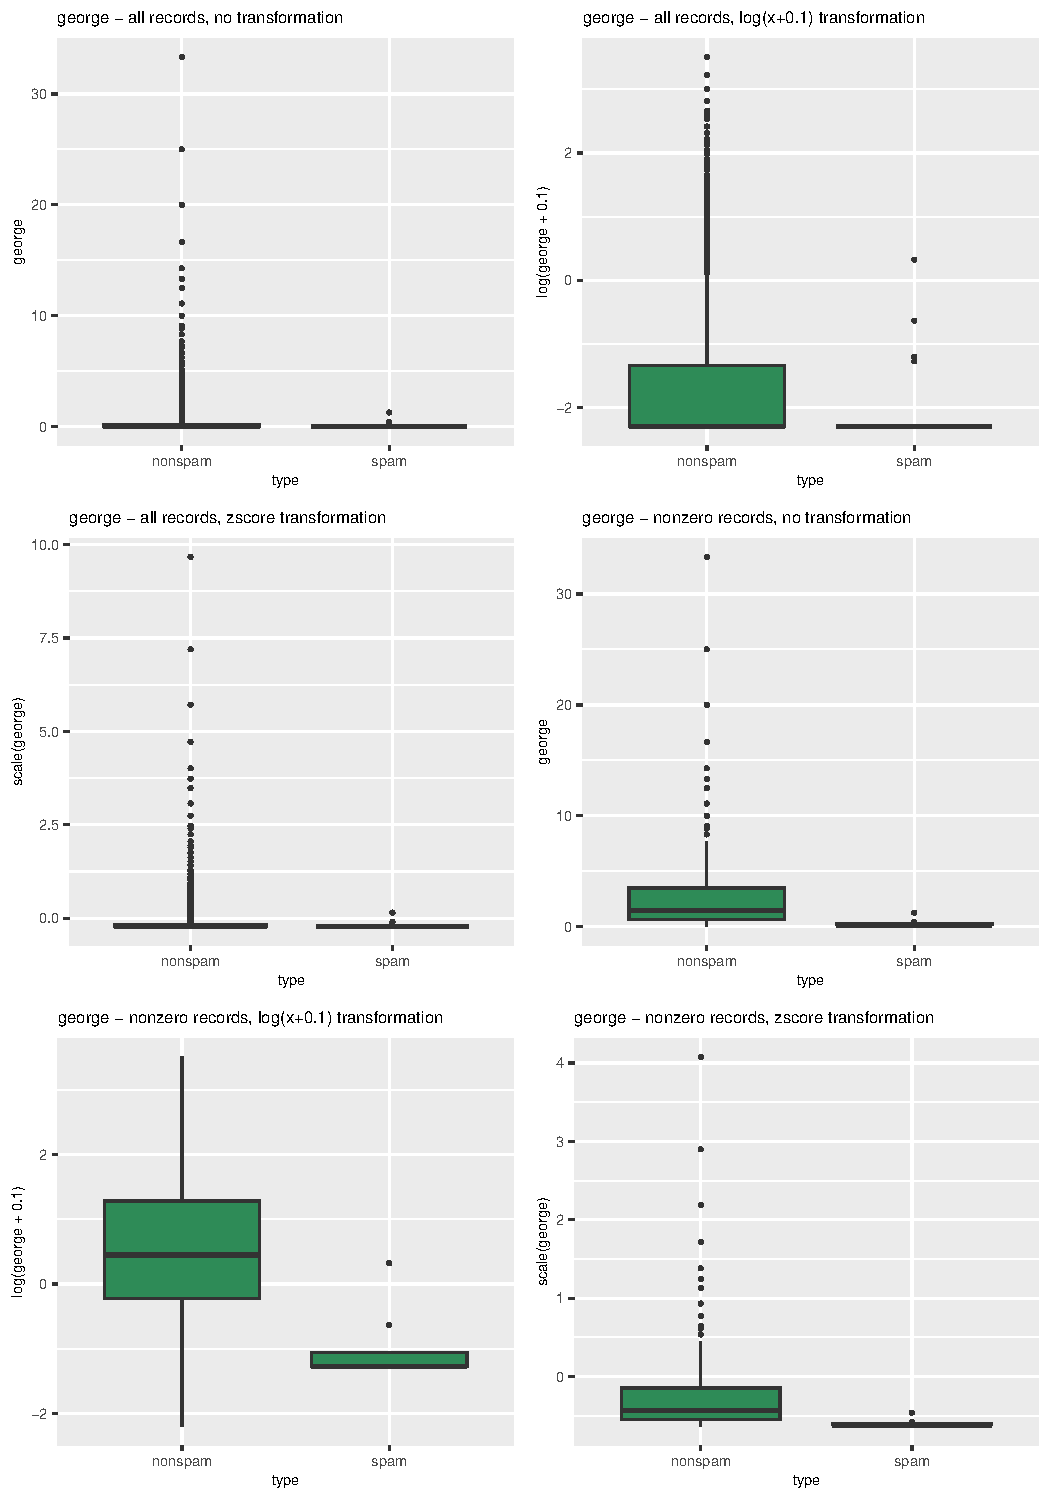
\includegraphics[width=\maxwidth]{figure/georgeBox-1} \caption[\label{fig2} Boxplots for george variable]{\label{fig2} Boxplots for george variable}\label{fig:georgeBox}
\end{figure}

\end{knitrout}

\begin{knitrout}
\definecolor{shadecolor}{rgb}{0.969, 0.969, 0.969}\color{fgcolor}\begin{figure}[h]
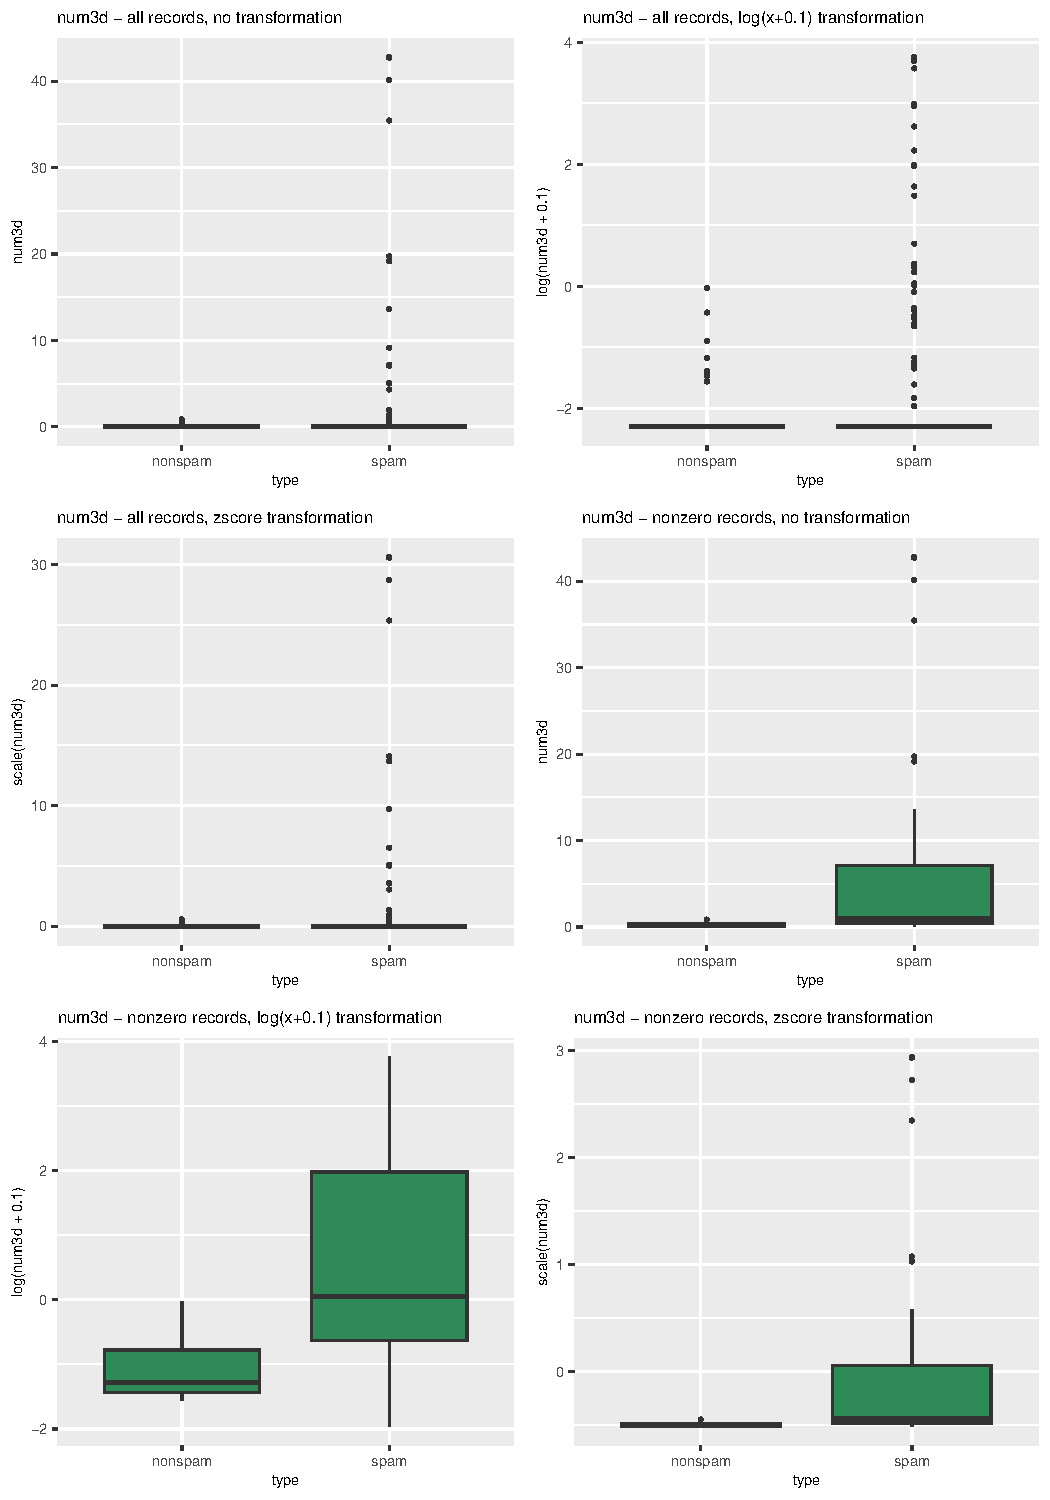
\includegraphics[width=\maxwidth]{figure/num3dBox-1} \caption[\label{fig3} Boxplots for num3d variable]{\label{fig3} Boxplots for num3d variable}\label{fig:num3dBox}
\end{figure}

\end{knitrout}

\begin{knitrout}
\definecolor{shadecolor}{rgb}{0.969, 0.969, 0.969}\color{fgcolor}\begin{figure}[h]
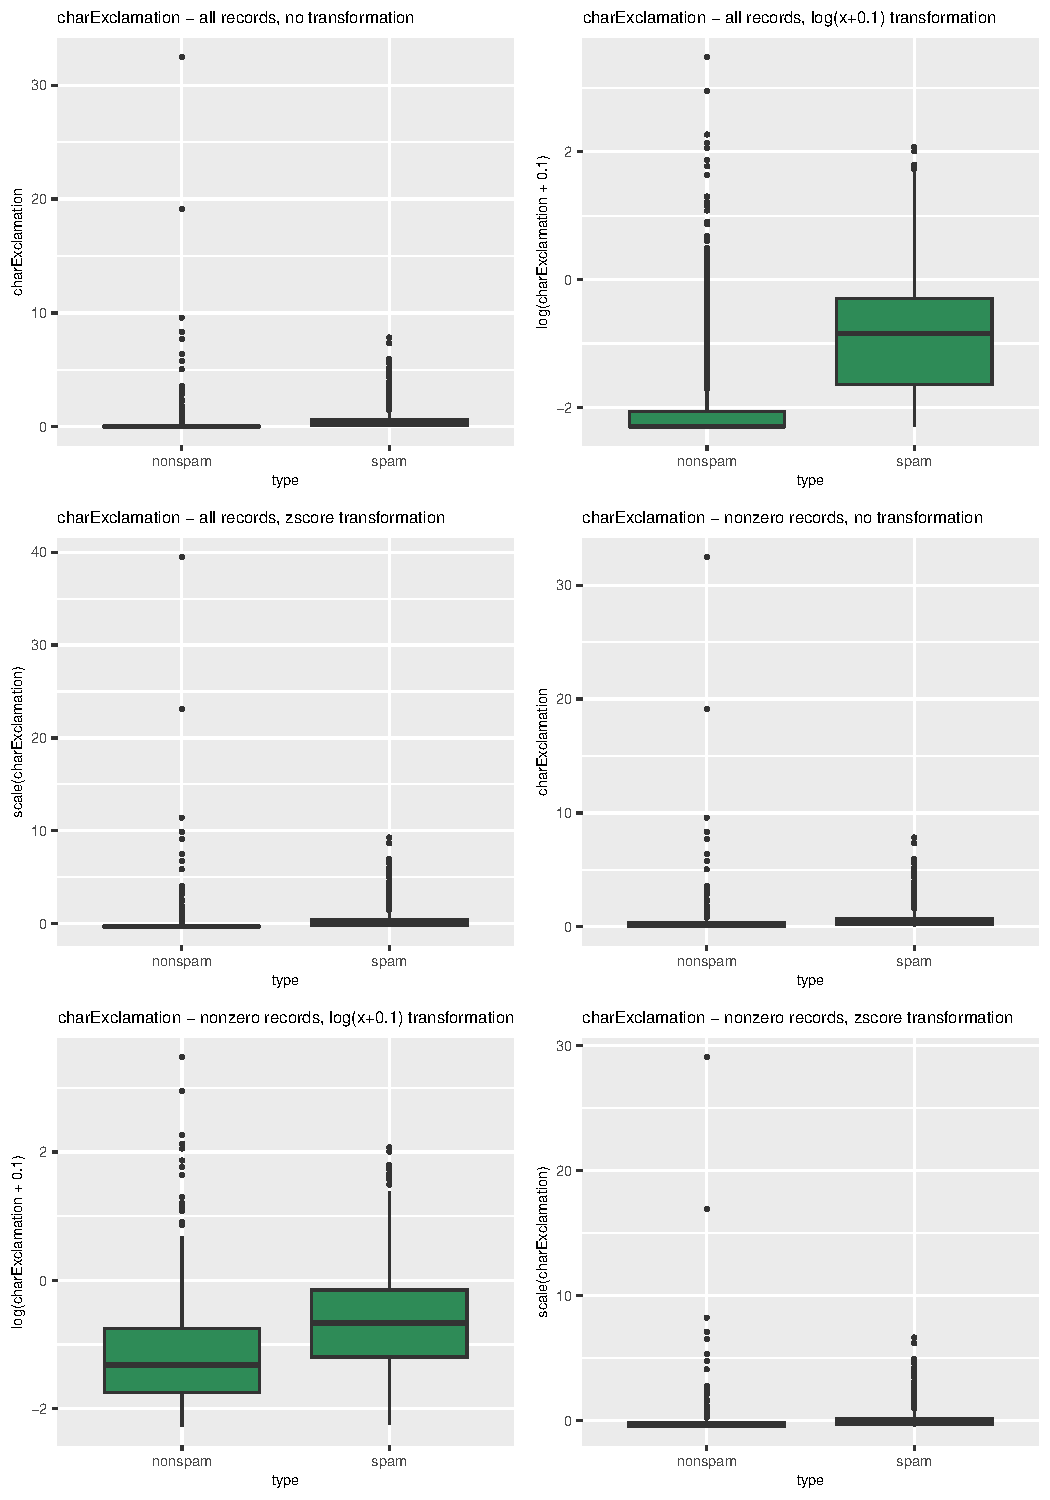
\includegraphics[width=\maxwidth]{figure/charExclamationBox-1} \caption[\label{fig4} Boxplots for charExclamation variable]{\label{fig4} Boxplots for charExclamation variable}\label{fig:charExclamationBox}
\end{figure}

\end{knitrout}

Figure \ref{fig2} shows the boxplots for \textit{george} variable. We can see that for the untransformed
data there are multiple outliers in the \textit{nonspam} class, few outliers for \textit{spam}, and
the distribution for both classes is strongly concentrated around zero. For z-score it looks almost
identical, but in the case of log transformation, we can see that the distribution spreads 
out a little -- at least we can distinguish quartiles for the \textit{nonspam} class, and the number
of detected outliers decreases. The changes are even more visible when we consider only nonzero records.
Here, again the untransformed data and z-score are very similar, and the log transformation in this case
displays wider boxes with only two outliers visible for the \textit{spam} class.
A similar situation can be observed for the \textit{num3d} (Figure \ref{fig3}) variable. Although the differences
between the raw and transformed data are not that clear in case of all records, 
it becomes very obvious when we just consider the nonzero values. Z-score and untransformed data
are again very similar, while for the log transformation we have very wide boxes and no 
outliers. Same observations can be drawn from Figure \ref{fig4}, showing the boxplots
for \textit{charExclamation} variable, although this time, we were not able to achieve a distribution without any outliers,
even in the case of log transformation with nonzero records only. Still, this method
clearly outperformed the z-score, resulting in much wider boxes and longer whiskers,
with less values detected as outliers.

As for the Capital features, their distributions also characterize with having
very low $3^{rd}$ quartile compared to maximum observed value. However, this time 
the $1^{st}$, $2^{nd}$ and $3^{rd}$ quartile differ from one another, and the
minimum value for all three variables is 1, so we don't need to consider the nonzero
case while looking for potential outliers. Still, the distributions are very much concentrated
around some relatively small value, with numerous outliers spread out above that value,
so we'll consider exactly the same transformations for this set of features.

\begin{knitrout}
\definecolor{shadecolor}{rgb}{0.969, 0.969, 0.969}\color{fgcolor}\begin{figure}[h]
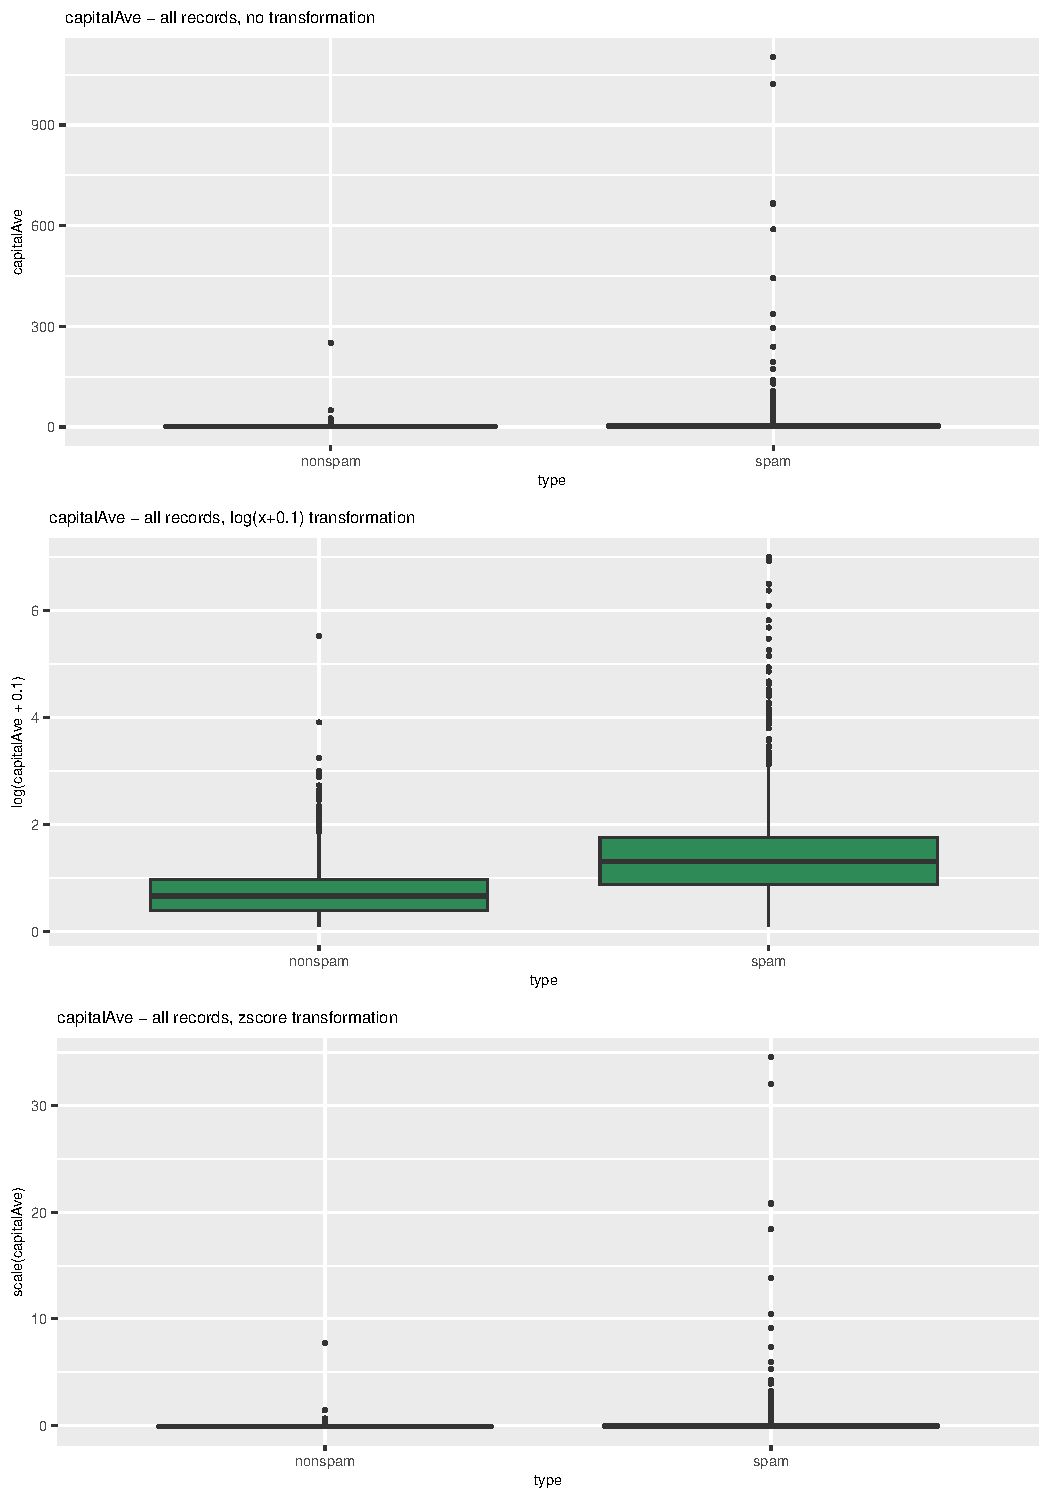
\includegraphics[width=\maxwidth]{figure/capitalAveBox-1} \caption[\label{fig5} Boxplots for capitalAve variable]{\label{fig5} Boxplots for capitalAve variable}\label{fig:capitalAveBox}
\end{figure}

\end{knitrout}

\begin{knitrout}
\definecolor{shadecolor}{rgb}{0.969, 0.969, 0.969}\color{fgcolor}\begin{figure}[h]
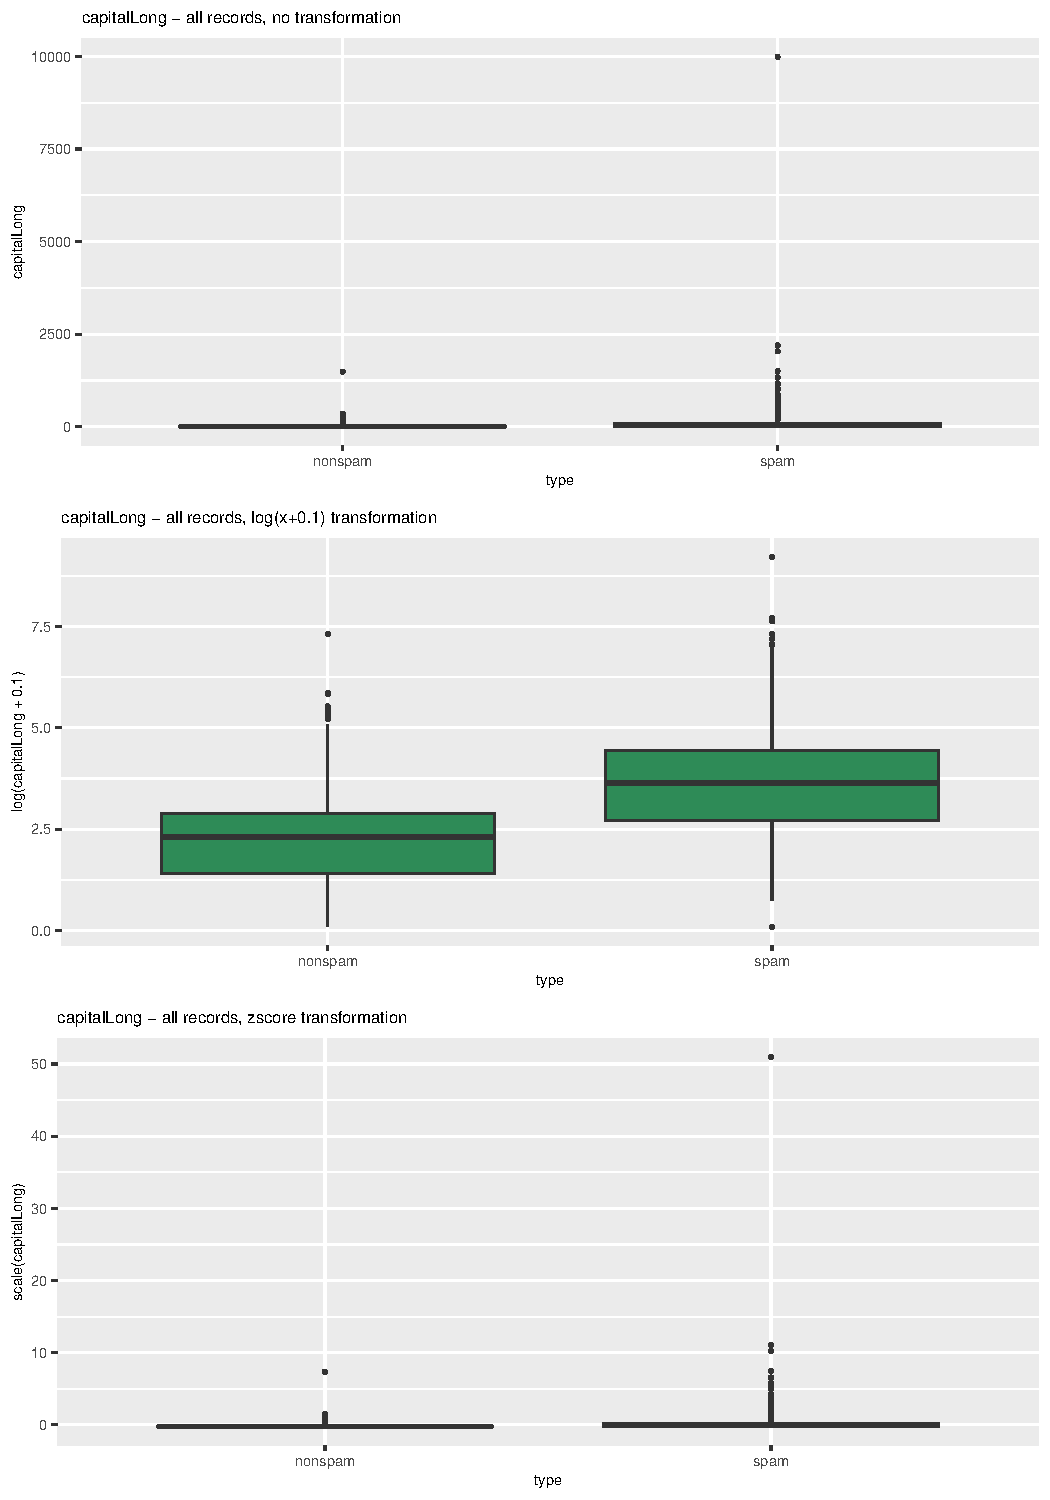
\includegraphics[width=\maxwidth]{figure/capitalLongBox-1} \caption[\label{fig6} Boxplots for capitalLong variable]{\label{fig6} Boxplots for capitalLong variable}\label{fig:capitalLongBox}
\end{figure}

\end{knitrout}

\begin{knitrout}
\definecolor{shadecolor}{rgb}{0.969, 0.969, 0.969}\color{fgcolor}\begin{figure}[h]
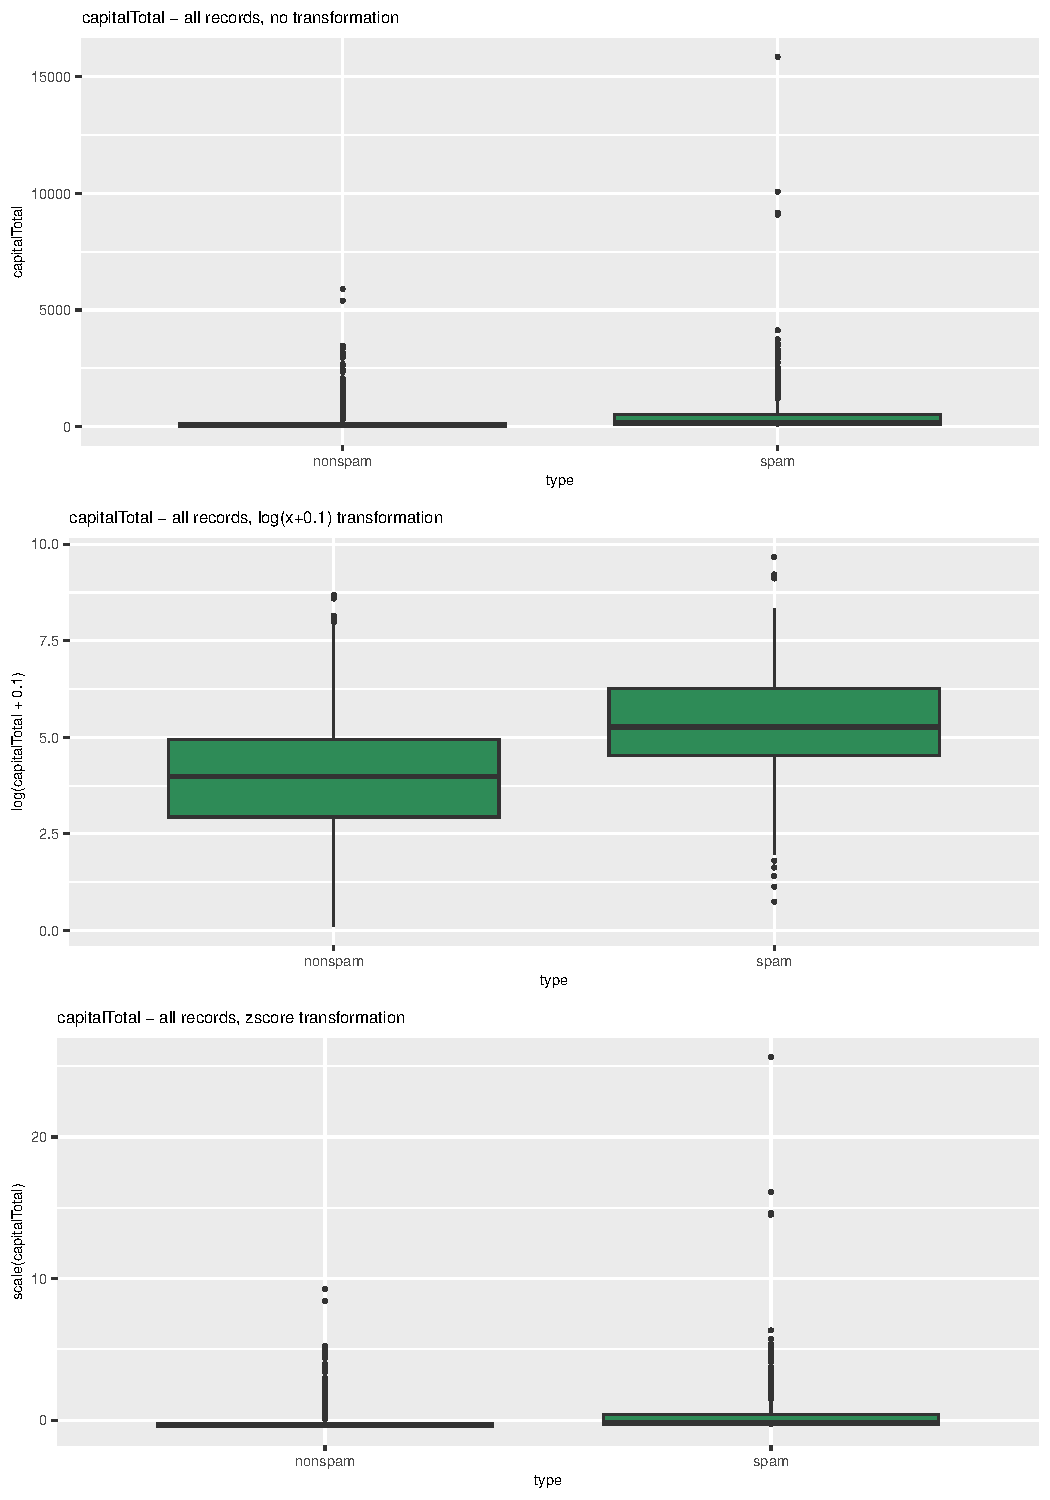
\includegraphics[width=\maxwidth]{figure/capitalTotalBox-1} \caption[\label{fig7} Boxplots for capitalTotal variable]{\label{fig7} Boxplots for capitalTotal variable}\label{fig:capitalTotalBox}
\end{figure}

\end{knitrout}

Let us first take a look at the \textit{capitalAve} variable boxplots, shown on Figure \ref{fig5}.
As in the previous cases, the log transformation stands out with wide boxes, but this time the number 
of outliers does not seem to be significantly decreased. For the \textit{capitalLong}
(Figure \ref{fig6}) and \textit{capitalTotal} (Figure \ref{fig7}), the results of 
log transformation are even better, reducing the number of potential outliers compared
to z-score and untransformed data.

To sum up, as the $log(x+0.1)$ data transformation seems to work better in most cases 
than the z-score standardization in case of reshaping the feature distribution, 
we expect that the classifiers will perform better on such transformed data. 
However, we are going to validate it later in this report by comparing the performance
of classification models using both methods.

\clearpage

\subsection*{Feature correlation}

The \textit{spambase} data set has as much as $57$ features, so elimination of some of those may 
have a significant impact on efficiency of classification algorithms. 
The most common approach here is to look at feature correlations. This way we can 
remove some variables that are highly correlated with others, as they do not provide 
much more information in the classification problem. It is also faster and more 
convenient to use only one of such variables. First let us take a look at correlation matrix, 
that was presented on Figure \ref{fig8} as it can show some interesting details about the data set.

\begin{knitrout}
\definecolor{shadecolor}{rgb}{0.969, 0.969, 0.969}\color{fgcolor}\begin{figure}[h]
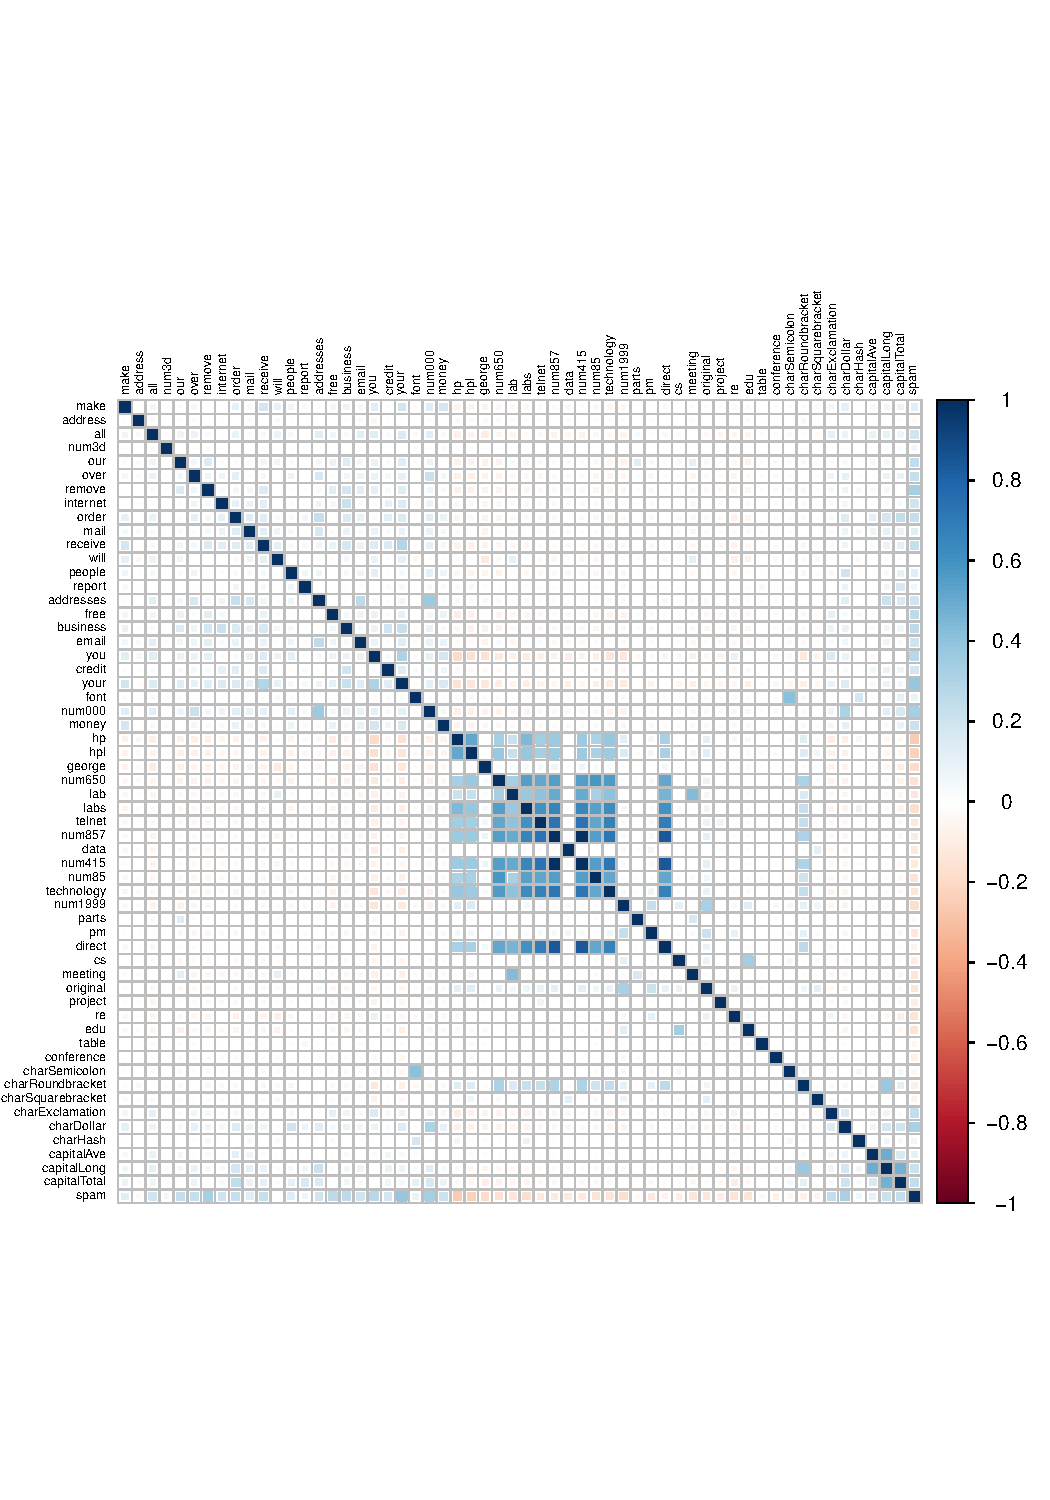
\includegraphics[width=\maxwidth]{figure/corrMatrix-1} \caption[\label{fig8} Correlation matrix of spam dataset]{\label{fig8} Correlation matrix of spam dataset}\label{fig:corrMatrix}
\end{figure}

\end{knitrout}

From the correlation matrix we see that there are a few features highly correlated 
with one another. However generally the explanatory variables don't seem to be highly correlated, 
so we expect that not many variables can be skipped in the later analysis. 
To check that further we use function $\texttt{findCorrelation}$ from \textit{caret} package, with cutoff equal to $0.8$.
\begin{knitrout}
\definecolor{shadecolor}{rgb}{0.969, 0.969, 0.969}\color{fgcolor}\begin{kframe}
\begin{verbatim}
## Compare row 32  and column  34 with corr  0.996 
##   Means:  0.143 vs 0.059 so flagging column 32 
## Compare row 34  and column  40 with corr  0.845 
##   Means:  0.127 vs 0.057 so flagging column 34 
## All correlations <= 0.8
\end{verbatim}
\end{kframe}
\end{knitrout}
From the output we can see that with adopted cutoff we can eliminate features \textit{num415} 
and \textit{num857}, so now we are left with $55$ variables. This is not the only advantage 
that correlation matrix can give us. We can also find variables that have the highest 
correlation with e-mail type. As the correlation matrix presented earlier is not easy to read, 
let us take out the features that have highest positive or negative correlation with type.



% latex table generated in R 4.3.1 by xtable 1.8-4 package
% Wed Dec  6 19:58:40 2023
\begin{table}[ht]
\centering
\begin{tabular}{rr}
  \hline
 & correlation\_with\_spam \\ 
  \hline
your & 0.38 \\ 
  num000 & 0.33 \\ 
  remove & 0.33 \\ 
  charDollar & 0.32 \\ 
  you & 0.27 \\ 
  free & 0.26 \\ 
  business & 0.26 \\ 
  hp & 0.26 \\ 
  capitalTotal & 0.25 \\ 
  our & 0.24 \\ 
   \hline
\end{tabular}
\caption{Features most correlated with target class variable} 
\label{tab2}
\end{table}


We can see that results from correlation matrix are confirmed in the above table with features highly correlated with \textit{type}. It's important to point 
out that those features may have a great impact on classification of e-mails,
which we will try to investigate later on.
	
\subsection*{Average frequency}
	
Other important data feature is the average value. In the classification problem 
the average value among all variables is not as interesting as its difference between 
two investigated types. Let us take out words and characters, whose frequencies 
demonstrate the highest difference in average value.

% latex table generated in R 4.3.1 by xtable 1.8-4 package
% Wed Dec  6 19:58:40 2023
\begin{table}[ht]
\centering
\begin{tabular}{rlrrrrrrrrrr}
  \hline
 & type & george & you & your & hp & free & hpl & charExclamation & our & re & edu \\ 
  \hline
1 & spam & 0.00 & 2.26 & 1.38 & 0.02 & 0.52 & 0.01 & 0.51 & 0.51 & 0.13 & 0.01 \\ 
  2 & nonspam & 1.27 & 1.27 & 0.44 & 0.90 & 0.07 & 0.43 & 0.11 & 0.18 & 0.42 & 0.29 \\ 
   \hline
\end{tabular}
\caption{Average frequency of variables across e-mail types} 
\label{tab3}
\end{table}


We expect that, as for features highly correlated with \textit{type}, those presented 
above will also have crucial impact on e-mail classification.

\clearpage

\section{Classification}

For the classification task, we will consider the complete dataset and several 
subsets of features and assess the accuracy for all of them. First, we want to check
how well Frequency features and Capital features perform when used separately. 
Then, we will examine if feature reduction to the features highly correlated with \textit{type}
or those with highest difference in average frequency between classes will lead 
to satisfactory results. Apart from comparing different feature subsets, we will also
inspect how the z-score scaling and $log(x+0.1)$ transformation will affect classification
outcome. Additionally, for the models that have the hyperparameters (KNN, Random Forest), we will tune them
using the 5-fold cross validation algorithm. To improve readability, the confusion matrices were moved to Section \ref{sec:appendix} (Appendix).

\subsection*{KNN}

Before approaching classification task with KNN, first we wanted to compute the average classification error
for two types of data transformations, and for $k \in \{1, 2, 3, \dots, 10\}$.
To do that, we performed 100 independent runs of train-test data split, training, prediction
and classification error calculation for each value of $k$ and each transformed dataset.
The results are displayed on Figure \ref{fig9}. We can see that the shape of both lines is similar,
with maximum at $k=2$, but the minimum for z-score is observed at $k=1$, and for $log(x+0.1)$
at $k=5$, which means that, on average, $k=2$ always performs the worst, but the best performing
value of $k$ depends on the data variant. Moreover, the error for log transformation is much smaller 
than for the z-score for all values of $k$, which suggests that we should rather use the 
log-transformed data for our classification task. Now we can check how KNN will perform with different sets of features,
each time using 5-fold cross validation algorithm to tune the optimal value of $k$.

\begin{knitrout}
\definecolor{shadecolor}{rgb}{0.969, 0.969, 0.969}\color{fgcolor}\begin{figure}[h]
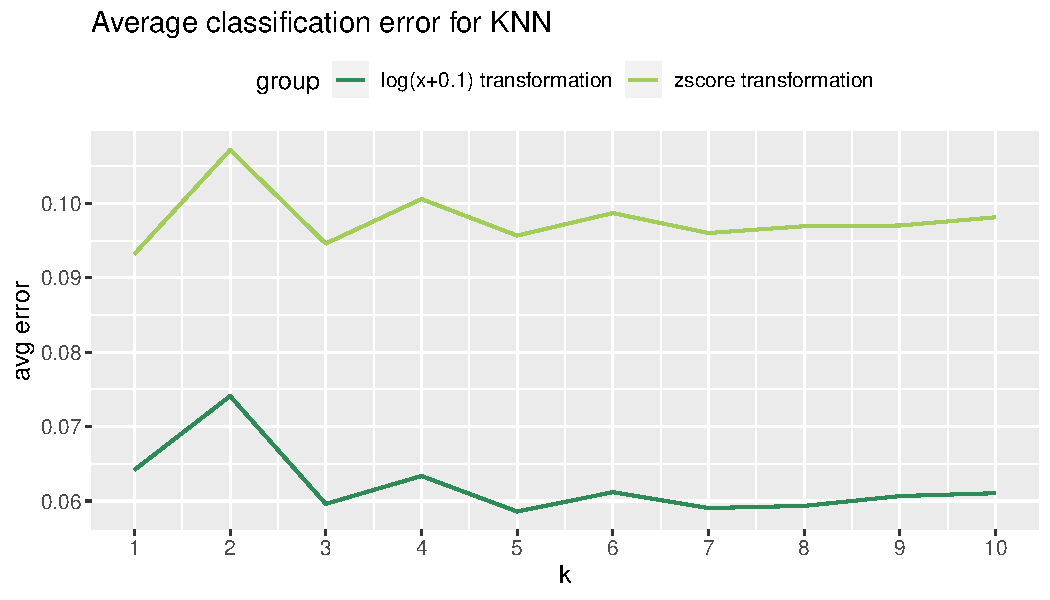
\includegraphics[width=\maxwidth]{figure/avgErrKNN-1} \caption[\label{fig9} Average classification error for KNN]{\label{fig9} Average classification error for KNN}\label{fig:avgErrKNN}
\end{figure}

\end{knitrout}

\subsubsection*{All features}

Table \ref{KNNcm1} shows the confusion matrix for all features KNN classification.
In this case, the algorithm picked $k=3$ as the optimal hyperparameter.
We see that most observations were classified correctly, resulting in 0.9391 accuracy,
0.9284 sensitivity and 0.9459 specificity, so the model performed slightly worse for 
the \textit{nonspam} class (we treat \textit{spam} as positive and \textit{nonspam} as negative).
Of course, the reason for that might be the slight class disproportion, as the model
had less observations of \textit{nonspam} to learn from.

\subsubsection*{Frequency features}

For Frequency features (Table \ref{KNNcm2}), we observe a worse performance, with 0.9287 accuracy,
0.9206 sensitivity and 0.9337 specificity. Again, the results are slightly better 
for the \textit{nonspam} class. Here, the optimal $k$ is again 3.

\subsubsection*{Capital features}

In the case of Capital features, the optimal value of $k$ is 1, and the KNN model performance goes down significantly
compared to the previous two sets of features. The observed accuracy is only 0.7991,
while the specificity is 0.8377, definitely outperforming the sensitivity
which is just 0.7413. We observe similar trend as in two cases described above, but 
this time much more obvious (see Table \ref{KNNcm3}).

\subsubsection*{Features highly correlated with \textit{type}}

Although it would seem that choosing the features highly correlated with target class variable
would lead to very good classification results, this is not the case for our data.
The confusion matrix, shown in Table \ref{KNNcm4}, looks very similar to that shown for the Capital features, 
and what follows, also the statistics are very close. This time we observe accuracy of
0.8070, sensitivity 0.7619 and specificity 0.8350. Optimal value of $k$ is 1.


\subsubsection*{Features with highest average difference in frequency between types}

The last set of features shows improvement over the previous two. Here, the accuracy is 0.9000,
sensitivity 0.8806 and specificity 0.9122 (see Table \ref{KNNcm5}). It is definitely not as good as in the case 
where we included all features or those related to frequency, but the difference is
not as significant as for the Capital features or the features highly correlated with \textit{type}.
The trend of better performance for the \textit{nonspam} class is preserved, and the 5-fold CV algorithm picked $k=10$.


\subsection*{Random Forest}

In case of Random Forest, we will follow the same procedure as for KNN -- first, 
we are going to look at the average classification error plot for both transformed
datasets, this time with \textit{mtry} parameter (number of features considered in each tree) on X-axis.
Athough the default number of trees for Random Forest in \textit{caret} is 500, we use only
100 trees, as it doesn't affect the results significantly.
The resulting plot is shown on Figure \ref{fig10}. This time it's not so easy to tell which data transformation
performed better. The lines intersect several times and none of them is clearly above the other.
However, the $\log(x+0.1)$ transformation resulted in smaller error around the
optimal value of \textit{mtry} ($\lfloor p \rfloor = 7$, $p$ -- number of features).
For that reason, and to keep consistent with the classifiers discussed earlier, 
we will use the log-transformed data for the classification task with Random Forest.

\begin{knitrout}
\definecolor{shadecolor}{rgb}{0.969, 0.969, 0.969}\color{fgcolor}\begin{figure}[h]
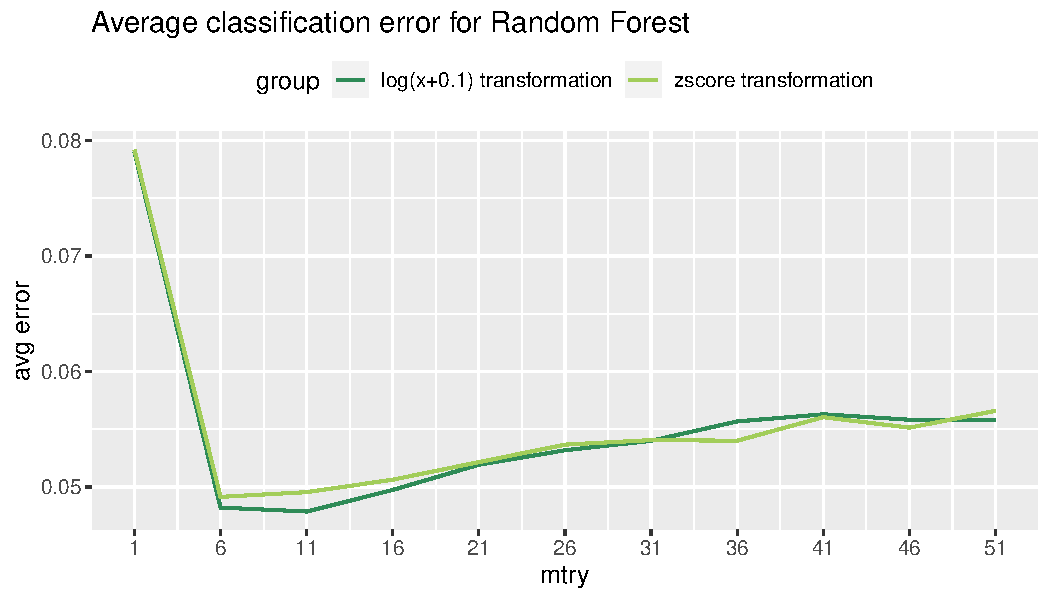
\includegraphics[width=\maxwidth]{figure/avgErrRF-1} \caption[\label{fig10} Average classification error for Random Forest]{\label{fig10} Average classification error for Random Forest}\label{fig:avgErrRF}
\end{figure}

\end{knitrout}

\subsubsection*{All features}

In case of all features Random Forest classification, the 5-fold CV algorithm picked 
6 as the optimal value of \textit{mtry}. The accuracy is 0.9470, which exceeds that 
of a KNN model, but not significantly (approximately 2\% difference).
The improvement is visible also with sensitivity (0.9537) and specificity (0.9429).
Contrary KNN, the model performed better for the \textit{spam} class.
The confusion matrix can be found in Table \ref{RFcm1}.

\subsubsection*{Frequency features}

After reducing the dataset to Frequency features only, we observe a very small decrease
in accuracy (0.9496). What's interesting, the sensitivity has decreased slightly,
reaching the value of 0.9519, while the specificity is better than for all features example,
being 0.9481 (see Table \ref{RFcm2}). The optimal value of \textit{mtry} is once again 6.

\subsubsection*{Capital features}

For the Capital features, the optimal value of \textit{mtry} turned out to be 1.
We observe a significant decrease of the model performance in this case. 
From confusion matrix, shown in Table \ref{RFcm3}, we can see that the accuracy
is 0.8278, the sensitivity is 0.8102 and the specificity is 0.8376. Those results 
are better than for the KNN run on the same set of features, but for sure we would 
not call them satisfying. What's worth noticing, the trend favoring the \textit{spam}
class that we observed for all other cases, is reversed here.

\subsubsection*{Features highly correlated with \textit{type}}

As opposed to KNN, in case of Random Forest we don't observe a significant decrease
of model performance after selecting the features highly correlated with \textit{type}.
The accuracy here is 0.9296, the sensitivity is 0.9189, and the specificity is 0.9363 (see Table \ref{RFcm4}).
Those results are slightly worse than for all features or Frequency features, but
still quite good. The optimal value of \textit{mtry} is 3 this time.
Again, the model performed better for the \textit{nonspam} class.


\subsubsection*{Features with highest average difference in frequency between types}

For the last set of features, the 5-fold CV algorithm picked 5 as the optimal
value of \textit{mtry}. As we can see from the confusion matrix shown in Table \ref{RFcm5},
the model performance is slightly worse than in case of
the previous set, but definitely better than for the Capital features,
giving accuracy of 0.9183. The sensitivity is 0.9224 and the specificity equals 0.9159.

\subsection*{Discriminant analysis}
Another useful classification algorithm is discriminant analysis. In this section 
we will use linear and quadratic discriminant analysis to determine e-mail type. This time there's no parameter tuning needed, so we will compare results for all features between data with z-score scaling and $log(x+0.1)$ transformation.
	
\subsection*{All features}

To compare results we again use the confusion matrix, first for scaled data we have Table 
\ref{tab:confusion_matrix_lda1} and Table \ref{tab:confusion_matrix_qda1}.
The accuracy for described methods is quite satisfying, for LDA it's $0.8904$ 
and for QDA - $0.847$. So in this case linear method works significantly better. 
There's also a disproportion in confusion matrices for those methods. LDA works in favor 
of spam messages, opposite situation occurs for QDA. Those features are nicely represented with sensitivity 
and specificity, that for LDA are respectively $0.9098$, $0.8802$ and for QDA: $0.7336$, $0.9677$. 

We perform the same algorithms on the data with log transformation and 
obtain Tables \ref{tab:confusion_matrix_lda1_log} and \ref{tab:confusion_matrix_qda1_log}.
We see that this transformation helped our algorithm to obtain better accuracy: 
$0.9348$ for LDA and $0.8574$ for QDA. As previously, we observe similar disproportion in
both methods, resulting in sensitivity 0.9479, specificity 0.9279 for LDA, and
respectively 0.7549, 0.9571. From that we conclude that other feature 
subsets will be tested for log transformed data.

\subsection*{Frequency features}

We again provide the confusion matrices that describe the classification methods: 
Table \ref{tab:confusion_matrix_lda2} and Table \ref{tab:confusion_matrix_qda2}.
Above results exhibit accuracy $0.9278$ for LDA and $0.853$ for QDA. We also 
observe similar disproportion in characteristics as for the previous case with 
$0.9363$ sensitivity and $0.9229$ specificity for LDA and respectively $0.7474$ 
and $0.9583$ for QDA. As we see elimination of features describing capital letters 
didn't have an enormous impact on discriminant analysis results.

\subsection*{Capital features}

This time we take into account only three features containing information about capital 
letters and get Tables \ref{tab:confusion_matrix_lda3} and \ref{tab:confusion_matrix_qda3}.
Here, similarly as for KNN and random forest methods, we obtain much worse accuracy: $0.7304$ for LDA and $0.7148$ - QDA. What's 
interesting is that this time the disproportion between wrong classification of 
different discriminant analysis algorithms is not that high. This results in sensitivity 
$0.7061$ and specificity $0.7410$ for LDA and $0.7254$, $0.7148$ respectively for QDA.

\subsection*{Features highly correlated with \textit{type}}
	 
LDA and QDA results are presented in Table \ref{tab:confusion_matrix_lda4} 
and Table \ref{tab:confusion_matrix_qda4}.
Despite having much less explanatory variables than when taking all frequency 
features we obtain similar accuracy: $0.8391$ - LDA and $0.8530$ - QDA. It's also 
important to note that QDA accuracy is almost as high as for all features. 
This variable selection also omits the disproportions 
between two analyzed discriminant analysis methods. Such property results in similar 
statistics for both of them. Namely $0.8807$ sensitivity and $0.8208$ specificity 
for LDA, $0.8817$ and $0.8393$ respectively for QDA.
	 
\subsection*{Features with highest average difference in frequency between types}
	 
Last feature selection that we test is for variables exhibiting highest difference in 
average frequency between types. Confusion matrices are shown in Table 
\ref{tab:confusion_matrix_lda5} ad Table \ref{tab:confusion_matrix_qda5}.
In this case accuracy of LDA is still comparable to other feature subsets, namely 
$0.8887$, however for QDA we get $0.793$. It means that this feature subset didn't 
have much impact on linear method, but for quadratic one it displays much worse accuracy. 
Also for QDA the disproportion between sensitivity and specificity is significant: 
$0.6646$ and $0.9618$ respectively. For LDA the disproportion is much smaller: 
$0.877$ - sensitivity and $0.8957$ - specificity.


\section{Conclusions}

The project focused on spam e-mail classification, covering Exploratory Data Analysis, 
feature selection, and the evaluation of classification algorithms.
Notable findings include the impact of various data transformations and the 
significance of choosing different feature subsets for classification models.
All the algorithms were quite responsive to variable selection. On general, 
the worst performing subset was Capital features, while the best performance was
achieved by using all explanatory variables or Frequency features.
What's interesting, reducing the number of columns from $55$ even to $10$, usually
didn't result in a significant drop in accuracy. 

When it comes to algorithmic performance, KNN's sensitivity to data transformation 
was evident, with log transformation consistently outperforming z-score scaling for all values of $k$. 
On the contrary, for the Random Forest the difference between the two data transformations
was not that clear, however the log-transformation was chosen as the better one as it
displayed smaller classification error for the optimal value of \textit{mtry} parameter.
Random Forest's performance persistently exceeded that of KNN, LDA and QDA, achieving higher accuracy, 
sensitivity, and specificity for all feature subsets. Moreover, KNN usually displayed better specificity,
while for the Random Forest situation was opposite for most cases.

Discriminant analysis, contrary to KNN and Random Forest, exhibited high disproportions 
between specificity and sensitivity. For LDA, better sensitivity is observed in 
most cases, while for QDA the specificity was usually higher, especially in the 
case of all features. Again, the comparison of scaled and log-transformed data 
highlighted the effectiveness of log transformation in enhancing classification accuracy.
Additionally, the QDA falls behind all other considered algorithms.

Above conclusions highlight the importance of strategic feature selection and data 
transformation for optimal classification results. For the future research, one
could consider the deep learning approach for spam classification, such as various
types of neural networks. On top of that, one could use the cost matrix to deploy
the cost-sensitive learning approach. Of course, the challenge here could be 
determining which e-mail type misclassification should be assigned with higher cost.
Additionally, the cluster analysis could be used to separate the data, which
will be done in the next part of the project.

\clearpage

\section{Appendix}
\label{sec:appendix}

\begin{table}[h]
    \centering
    \begin{tabular}{lcc}
        & \textbf{Reference} & \\
        \textbf{Prediction} & nonspam & spam \\
        nonspam & 665 & 32 \\
        spam & 38 & 415 \\
    \end{tabular}
    \caption{Confusion matrix - KNN, all features}
    \label{KNNcm1}
\end{table}

\begin{table}[h]
    \centering
    \begin{tabular}{lcc}
        & \textbf{Reference} & \\
        \textbf{Prediction} & nonspam & spam \\
        nonspam & 662 & 35 \\
        spam & 47 & 406 \\
    \end{tabular}
    \caption{Confusion matrix - KNN, Frequency features}
    \label{KNNcm2}
\end{table}

\begin{table}[h]
    \centering
    \begin{tabular}{lcc}
        & \textbf{Reference} & \\
        \textbf{Prediction} & nonspam & spam \\
        nonspam & 578 & 119 \\
        spam & 112 & 341 \\
    \end{tabular}
    \caption{Confusion matrix - KNN, Capital features}
    \label{KNNcm3}
\end{table}

\begin{table}[h]
    \centering
    \begin{tabular}{lcc}
        & \textbf{Reference} & \\
        \textbf{Prediction} & nonspam & spam \\
        nonspam & 592 & 105 \\
        spam & 117 & 336 \\
    \end{tabular}
    \caption{Confusion matrix - KNN, Features highly correlated with type}
    \label{KNNcm4}
\end{table}

\begin{table}[h]
    \centering
    \begin{tabular}{lcc}
        & \textbf{Reference} & \\
        \textbf{Prediction} & nonspam & spam \\
        nonspam & 644 & 53 \\
        spam & 62 & 391 \\
    \end{tabular}
    \caption{Confusion matrix - KNN, Features with highest average difference in frequency between types}
    \label{KNNcm5}
\end{table}

\begin{table}[h]
    \centering
    \begin{tabular}{lcc}
        & \textbf{Reference} & \\
        \textbf{Prediction} & nonspam & spam \\
        nonspam & 677 & 20 \\
        spam & 41 & 412 \\
    \end{tabular}
    \caption{Confusion matrix - Random Forest, all features}
    \label{RFcm1}
\end{table}

\begin{table}[h]
    \centering
    \begin{tabular}{lcc}
        & \textbf{Reference} & \\
        \textbf{Prediction} & nonspam & spam \\
        nonspam & 676 & 21 \\
        spam & 37 & 416 \\
    \end{tabular}
    \caption{Confusion matrix - Random Forest, Frequency features}
    \label{RFcm2}
\end{table}

\begin{table}[h]
    \centering
    \begin{tabular}{lcc}
        & \textbf{Reference} & \\
        \textbf{Prediction} & nonspam & spam \\
        nonspam & 619 & 78 \\
        spam & 120 & 333 \\
    \end{tabular}
    \caption{Confusion matrix - Random Forest, Capital features}
    \label{RFcm3}
\end{table}

\begin{table}[h]
    \centering
    \begin{tabular}{lcc}
        & \textbf{Reference} & \\
        \textbf{Prediction} & nonspam & spam \\
        nonspam & 661 & 36 \\
        spam & 45 & 408 \\
    \end{tabular}
    \caption{Confusion matrix - Random Forest, Features highly correlated with type}
    \label{RFcm4}
\end{table}

\begin{table}[h]
    \centering
    \begin{tabular}{lcc}
        & \textbf{Reference} & \\
        \textbf{Prediction} & nonspam & spam \\
        nonspam & 664 & 33 \\
        spam & 61 & 392 \\
    \end{tabular}
    \caption{Confusion matrix - Random Forest, Features with highest average difference in frequency between types}
    \label{RFcm5}
\end{table}

\begin{table}[h]
	\centering
	\begin{tabular}{lcc}
		& \textbf{Reference} & \\
		\textbf{Prediction} & nonspam & spam \\
		nonspam & 661 & 36 \\
		spam & 90 & 363 \\
	\end{tabular}
	\caption{Confusion Matrix - LDA, all features, scaled data}
	\label{tab:confusion_matrix_lda1}
\end{table}

\begin{table}[h]
	\centering
	\begin{tabular}{lcc}
		& \textbf{Reference} & \\
		\textbf{Prediction} & nonspam & spam \\
		nonspam & 539 & 158 \\
		spam & 18 & 435 \\
	\end{tabular}
	\caption{Confusion Matrix - QDA, all features, scaled data}
	\label{tab:confusion_matrix_qda1}
\end{table}

\begin{table}[h]
	\centering
	\begin{tabular}{lcc}
		& \textbf{Reference} & \\
		\textbf{Prediction} & nonspam & spam \\
		nonspam & 675 & 22 \\
		spam & 53 & 400 \\
	\end{tabular}
	\caption{Confusion Matrix - LDA, all features, log data}
	\label{tab:confusion_matrix_lda1_log}
\end{table}

\begin{table}[h]
	\centering
	\begin{tabular}{lcc}
		& \textbf{Reference} & \\
		\textbf{Prediction} & nonspam & spam \\
		nonspam & 558 & 139 \\
		spam & 25 & 428 \\
	\end{tabular}
	\caption{Confusion Matrix - QDA, all features, log data}
	\label{tab:confusion_matrix_qda1_log}
\end{table}

\begin{table}[h]
	\centering
	\begin{tabular}{lcc}
		& \textbf{Reference} & \\
		\textbf{Prediction} & nonspam & spam \\
		nonspam & 670 & 27 \\
		spam & 56 & 397 \\
	\end{tabular}
	\caption{Confusion Matrix - LDA, frequency features}
	\label{tab:confusion_matrix_lda2}
\end{table}

\begin{table}[h]
	\centering
	\begin{tabular}{lcc}
		& \textbf{Reference} & \\
		\textbf{Prediction} & nonspam & spam \\
		nonspam & 552 & 145 \\
		spam & 24 & 429 \\
	\end{tabular}
	\caption{Confusion Matrix - QDA, frequency features}
	\label{tab:confusion_matrix_qda2}
\end{table}

\begin{table}[h]
	\centering
	\begin{tabular}{lcc}
		& \textbf{Reference} & \\
		\textbf{Prediction} & nonspam & spam \\
		nonspam & 595 & 102 \\
		spam & 208 & 245 \\
	\end{tabular}
	\caption{Confusion Matrix - LDA, capital features}
	\label{tab:confusion_matrix_lda3}
\end{table}

\begin{table}[h]
	\centering
	\begin{tabular}{lcc}
		& \textbf{Reference} & \\
		\textbf{Prediction} & nonspam & spam \\
		nonspam & 619 & 78 \\
		spam & 247 & 206 \\
	\end{tabular}
	\caption{Confusion Matrix - QDA, capital features}
	\label{tab:confusion_matrix_qda3}
\end{table}

\begin{table}[h]
	\centering
	\begin{tabular}{lcc}
		& \textbf{Reference} & \\
		\textbf{Prediction} & nonspam & spam \\
		nonspam & 655 & 42 \\
		spam & 143 & 310 \\
	\end{tabular}
	\caption{Confusion Matrix - LDA, features correlated with type}
	\label{tab:confusion_matrix_lda4}
\end{table}

\begin{table}[h]
	\centering
	\begin{tabular}{lcc}
		& \textbf{Reference} & \\
		\textbf{Prediction} & nonspam & spam \\
		nonspam & 653 & 44 \\
		spam & 125 & 328 \\
	\end{tabular}
	\caption{Confusion Matrix - QDA, features correlated with type}
	\label{tab:confusion_matrix_qda4}
\end{table}

\begin{table}[h]
 	\centering
 	\begin{tabular}{lcc}
 		& \textbf{Reference} & \\
 		\textbf{Prediction} & nonspam & spam \\
 		nonspam & 644 & 53 \\
 		spam & 75 & 378 \\
 	\end{tabular}
 	\caption{Confusion Matrix - LDA, features with highest average difference in}
 	\label{tab:confusion_matrix_lda5}
 \end{table}
 
 \begin{table}[h]
 	\centering
 	\begin{tabular}{lcc}
 		& \textbf{Reference} & \\
 		\textbf{Prediction} & nonspam & spam \\
 		nonspam & 478 & 219 \\
 		spam & 19 & 434 \\
 	\end{tabular}
 	\caption{Confusion Matrix - QDA, features with highest average difference in}
 	\label{tab:confusion_matrix_qda5}
\end{table}


\end{document}
